\documentclass{article}
\usepackage[utf8]{inputenc}
\usepackage{graphicx}
\usepackage{enumitem}
\usepackage{siunitx}
\usepackage{multirow}
\usepackage[a4paper, total={6in, 8in}]{geometry}
\usepackage[style=authoryear-ibid,backend=biber]{biblatex}
\usepackage[swedish]{babel}
\usepackage{float}
\usepackage{caption}
\usepackage[parfill]{parskip}
\usepackage{amsmath}
\usepackage{csquotes}
\usepackage{comment}
\usepackage{url}


\graphicspath{ {img/} }

\title{\Huge Operating Systems - Study \\ EDAF35}
%\author{\Large Elias Bergström, Emma Lindh, Elin Helmersson, Shahriar Chegini}
\author{  
    Elias Bergström\\
    \texttt{el8025be-s@student.lu.se}
    }
%\date{VT2024}
\date{\today}

\renewcommand{\figurename}{Figur}
\renewcommand{\tablename}{Tabell}

%handledarens namn

\begin{document}

\maketitle
\thispagestyle{empty}
%\pagenumbering{gobble}
\pagebreak
%\thispagestyle{empty}
%\pagenumbering{arabic}

\section{Module 2 - Processes and Threads}
\subsection{Red Box}
\begin{itemize}
    \item It is important to understand what the PCB is and that the PCBs get put on different queues by the OS when
    managing process state.
    (From section 3.1.3 to the end of 3.2.1 in Operating System Concepts)
    \item You need to understand process creation (including fork() and exec() in detail) and process termination (including
    zombie and orphan processes). From section 3.1.3 to the end of 3.2.1 in Operating System Concepts)
    \item You need to understand the difference between user threads and kernel threads and the different models for
    mapping between the two (Section 4.3 in Operating System Concepts)
\end{itemize}

\subsection{Notes}



The process can be in a number of different states, see figure.

\begin{figure}[H]
    \centering
    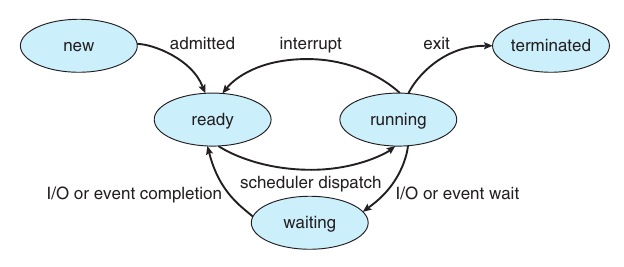
\includegraphics[width=0.8\textwidth]{pcb.png}
    \caption{Diagram of process states}
    \label{fig:diapcb}
\end{figure}


\subsubsection{PCB}
PCB stands for Process Control Block and each process is represented in the OS by one. The PCB contains information about the process:
\begin{itemize}
    \item {\bf Process state.} The state may be new, ready, running, waiting, halted, and
    so on.
    \item {\bf Program counter.} The counter indicates the address of the next instruction
    to be executed for this process.
    \item {\bf CPU registers.}
    \item {\bf CPU-scheduling information.} This information includes a process prior-
    ity, pointers to scheduling queues, and any other scheduling parameters.
    (Chapter 5 describes process scheduling.)
    \item {\bf Memory-management information.} This information may include such
    items as the value of the base and limit registers and the page tables, or the
    segment tables, depending on the memory system used by the operating
    system (Chapter 9).
    \item {\bf Accounting information} This information includes the amount of CPU
    and real time used, time limits, account numbers, job or process numbers,
    and so on.
    \item {\bf I/O status information.} This information includes the list of I/O devices
    allocated to the process, a list of open files, and so on.
\end{itemize}
In brief, the PCB simply serves as the repository for all the data needed to start,
or restart, a process, along with some accounting data.

\subsection*{fork() and exec() in Unix/Linux Context}

In a Unix/Linux context, \texttt{fork()} and \texttt{exec()} are system calls used for process creation and management.

\subsubsection*{fork()}
The \texttt{fork()} system call creates a new process by duplicating the calling (parent) process. The new process is called the \textit{child} process. Both the parent and the child process continue executing from the point of the \texttt{fork()} call. The child process gets a copy of the parent’s memory space, but they have different Process IDs (PIDs). \texttt{fork()} returns:
\begin{itemize}
    \item \texttt{0} in the child process.
    \item The child’s PID in the parent process.
\end{itemize}

\subsubsection*{exec()}
The \texttt{exec()} family of functions (e.g., \texttt{execvp()}, \texttt{execp()}, etc.) replaces the current process’s memory space with a new program. After calling \texttt{exec()}, the process image is completely replaced, and the new program starts executing. This is commonly used after \texttt{fork()} when the child process needs to run a different program than the parent.

\subsubsection*{Typical Usage}
In typical usage:
\begin{enumerate}
    \item \texttt{fork()} is used to create a new process.
    \item \texttt{exec()} is used by the child (or parent) to replace its process image with a different program.
\end{enumerate}

Together, these calls enable the creation of new processes and the execution of different programs, which is fundamental for tasks like launching new applications or running shell commands.



\subsubsection{Multithreading Models}
These models describes how to map user thread to kernel threads. User threads are supported above the kernel and are managed without kernel support and the kernel threads are managed by the kernel.

\begin{itemize}
    \item {\bf Many-to-One Model}, all user threads are mapped to one kernel 
    thread, where the switching between threads are done by a thread library in user space (not by the kernel)
    It's efficient but if the current user threads hangs it will also hang the kernel thread.
    \item {\bf One-to-One Model}, maps each user thread to a kernel thread. Multiple threads can run at the same time. The problem with this model is that you need to create a kernel thread for each user thread.
    \item {\bf Many-to-Many}, multiplexs many user threads to a smaller or equal amount of kernel threads.
    \item {\bf Two-Level Model} mixing two of the models. 
\end{itemize}




\section{Module 3.A - CPU Scheduling}
\subsection{Red Box}
\begin{itemize}
    \item Make sure you understand what it means for scheduling to be pre-emptive.
    (From section 5.1.3 in Operating System Concepts)
    \item You need to know and understand the tradeoffs between these different algorithms
    (Section 5.3 in Operating System Concepts)
    \item Be able to understand the differences between process and system contention scopes
    (Section 5.4 in Operating System Concepts)
    \item You need to understand ready queues, load balancing and processor affinity in multiprocessor systems
    (Section 5.5.1, 5.5.3 and 5.5.4 ins Operating System Concepts)
    \item You need to understand what makes real time scheduling different, the periodic process model and the
    differences between the RMS and the EDF scheduler (Section 5.6.1 – 5.6.4 in Operating System Concepts)
\end{itemize}

\begin{enumerate}
    \item When a process switches from the running state to the waiting state (for
    example, as the result of an I/O request or an invocation of wait() for the
    termination of a child process)
    \item When a process switches from the running state to the ready state (for
    example, when an interrupt occurs)
    \item When a process switches from the waiting state to the ready state (for
    example, at completion of I/O)
    \item When a process terminates
\end{enumerate}

When scheduling takes place only under circumstances 1 and 4, we say that the scheduling scheme is non preemptive or cooperative.
Otherwise, it is {\bf preemptive}. 
\\
\\
Chatgpt says the following:
\\ {\it Preemptive scheduling is a CPU scheduling method where the operating system can interrupt a running process to give the CPU to another process, usually with higher priority or urgency.
In this system, the OS can stop a process and switch to another one, either after a fixed time slice (in round-robin scheduling) or if a higher-priority process needs the CPU.}

\subsection{Scheduling Algorithms}

\subsubsection{First-Come, First-Served Scheduling (FCFS)}
This is the simplest algorithm. With this scheme, the process that requests the
CPU first is allocated the CPU first. The implementation of the FCFS policy is
easily managed with a FIFO queue. When a process enters the ready queue, its
PCB is linked onto the tail of the queue. When the CPU is free, it is allocated to
the process at the head of the queue. The running process is then removed from
the queue. The code for FCFS scheduling is simple to write and understand.
On the negative side, the average waiting time under the FCFS policy is
often quite long. {\bf Pro: simplest Con: Can have long wait times}.

\subsubsection{Shortest-Job-First (SJF) Scheduling}
Do the shortest job first. If to jobs take the same time FCFS is used to break the tie.
The more appropriate term for this method is {\bf shortest-next-CPU-burst}, because scheduling depends on the length of the next CPU burst of
a process, rather than its total length. 


Although the SJF lagorithm is optimal, it cannot be implemented at the level of CPU scheduling, 
as there is no way to know the length of the next CPU burst.
One approach to this problem is to try to approximate SJF scheduling. We may
not know the length of the next CPU burst, but we may be able to predict its
value. We expect that the next CPU burst will be similar in length to the previous
ones. By computing an approximation of the length of the next CPU burst, we
can pick the process with the shortest predicted CPU burst.


{\bf Pro: less down time then FCFS Con: harder to implement.}

 
{\bf Whats the difference between Job and CPU burst?}


\subsubsection{Round-Robin (RR) Scheduling}

Similar to FCFS but with preemption added. 

To implement RR scheduling, we again treat the ready queue as a FIFO
queue of processes. New processes are added to the tail of the ready queue.
\\
The CPU scheduler picks the first process from the ready queue, sets a timer to
interrupt after 1 time quantum, and dispatches the process.
One of two things will then happen. The process may have a CPU burst of
less than 1 time quantum. In this case, the process itself will release the CPU
voluntarily. The scheduler will then proceed to the next process in the ready
queue. If the CPU burst of the currently running process is longer than 1 time
quantum, the timer will go off and will cause an interrupt to the operating
system. A context switch will be executed, and the process will be put at the
tail of the ready queue. The CPU scheduler will then select the next process in
the ready queue.
\\

{\bf Con: the average waiting time under RR is often long. Pro: Relatively simple.}


\subsubsection{Priority Scheduling}

SJF is a special case of the general priority-scheduling. 
\\
A priority is associated with each process, and the CPU is allocated to the process with the highest priority. Equal-priority processes are scheduled in
FCFS order. An SJF algorithm is simply a priority algorithm where the priority
(p) is the inverse of the (predicted) next CPU burst. The larger the CPU burst,
the lower the priority, and vice versa.
\\


{\bf Con: different systems have different levels of priority, i.e. code is not portable.}



\subsubsection{Multilevel Queue Scheduling}

Separate queues for different priority levels. Often use RR per queue.
\\
{\bf Pro: you don't need to do an O(n) search to find the task with the highest priority.}



\subsubsection{Multilevel Feedback Queue Scheduling}

It's the same as Multilevel Queue Scheduling, but tasks can move between queues. 



\subsection{Differences between process and system contention scopes.} %page 217

Process contention scope and system contention scope are two types of thread scheduling models used to determine 
how threads compete for CPU time. They define the level at which threads contend for CPU 
resources, either within a process or across the entire system.



\subsubsection{Process Contention Scope (PCS)}

\begin{itemize}
    \item {\bf Scope:} Threads within the same process contend for CPU time only with other threads of that same process.
    \item {\bf Scheduling:} Threads are scheduled based on the process's thread priority and its own internal scheduling policies. The OS doesn't consider other processes' threads when scheduling threads for a particular process.
    \item {\bf Example:}Example: If two threads are running in a single process, they compete for CPU time only with each other, without interference from threads of other processes.
\end{itemize}


\subsubsection{System Contention Scope (SCS)}

\begin{itemize}
    \item {\bf Scope:} Threads from all processes in the system compete for CPU time against each other, regardless of the process they belong to.
    \item {\bf Scheduling:} Threads are scheduled system-wide, with the OS considering all threads in the system, not just those within the same process.
    \item {\bf Example:} Threads from different processes (e.g., Thread A from Process 1 and Thread B from Process 2) compete for CPU time on the same level, meaning the OS schedules them based on their priority relative to each other.
\end{itemize}

In short, {\bf PCS} is more localized within a process, while {\bf SCS} involves all threads in the system competing for CPU time.





\section{Module 3.B - Synchronization}
\subsection{Red Box}
\begin{itemize}
    \item You should know what the critical section problem is (Section 6.2 in Operating System Concepts)
    \item You must know the differences between Spinlocks, Semaphores and Mutexes in the context of Operating
    (Systems. 6.5 and 6.6 in Operating System Concepts – not the clearest explanation. Chapter 9, 10 in Linux Kernel
    development )
\end{itemize}



\subsection{Critical Section Problem}

The critical-section problem is to design a protocol that the processes can use to 
synchronize their activity so as to cooperatively share data. I.E, when one process is executing in it's
critical section another process can't do the same.
\\
A solution to this problem must satisfy the following:

\begin{enumerate}
    \item {\bf Mutual exclusion.} If a process is executing in its critical section, then no
    other processes can be executing in their critical sections.
    \item {\bf Progress.} If no process is executing in its critical section and some pro-
    cesses wish to enter their critical sections, then only those processes that
    are not executing in their remainder sections can participate in deciding which 
    will enter its critical section next, and this selection cannot be
    postponed indefinitely.
    \item {\bf Bounded waiting.} There exists a bound, or limit, on the number of times
    that other processes are allowed to enter their critical sections after a
    process has made a request to enter its critical section and before that
    request is granted.
\end{enumerate}


%You must know the differences between Spinlocks, Semaphores and Mutexes in the context of Operating

\subsection{Different types of locks}

\begin{itemize}
    \item {\bf Mutexes.} A mutex (mutual exclusion) lock is a synchronization mechanism that ensures only one thread can 
    access a shared resource at a time, preventing race conditions. 
    When a thread locks the mutex, others must wait until it is released, 
    ensuring exclusive access and data integrity during concurrent operations.
    \item {\bf Spinlocks.} A type of mutex lock where the process "spins" (busy-waits) for acquire. 
    \item {\bf Semaphores.} A integer var that is access through two atomic operations: wait() and signal().
\end{itemize}





\section{Module 4 - Memory Management}
\subsection{Red Box}
\begin{itemize}
    \item You need to understand what the physical and logic address space is and the motivation behind it. You also need to understand that
    the mmu is required to translate between the two (9.1.1 to 9.1.4 in operating system concepts).
    \item You need to understand what contigous allocation is, how it works and why fragmentation is a major issue.
    (section 9.2 in operating system concepts)
    \item You need to understand what paging is, what the page table and tlb are,
    and have a general idea of what protection and shared
    pages are (section 9.2 in operating system concepts).
    \item You need to know why we cannot use simple page tables, the three alternative page table structures and the advantages and
    disadvantages of each (section 9.4 of operating system concepts).
    \item You need to understand the basic concepts of virtual memory and its advantages(section 10.1 of operating system concepts).
    \item You need to be able to explain what demand paging is, free frame list and its performance (section 10.2 of operating system concepts).
    \item You need to know what page replacement is, understand the main three different page replacement algorithms discussed in the book
    and their tradeoffs, and be able to describe belady’s anomaly (section 10.4 of operating system concepts).
\end{itemize}


\subsection{Physical and logic address space and MMU}

The physical address space refers to the actual addresses in the RAM (hardware memory), 
while the logical address space refers to the addresses used by programs during execution, 
which are mapped to physical addresses by the operating system.
\newline

{\bf Key differences:}
\begin{itemize}
    \item {\bf Physical Address:} Actual memory locations in RAM.
    \item {\bf Logical Address:} Virtual addresses used by programs.
    \item {\bf Mapping: } Logical addresses are mapped to physical addresses by the MMU.
\end{itemize}

{\bf Reason:}
\begin{itemize}
    \item {\bf Isolation \& Protection:} Logical addresses allow programs to operate in isolated, virtualized memory spaces, preventing interference between programs.
    \item {\bf Efficient Memory Use:} Virtual memory lets programs use more memory than physically available by swapping data between RAM and disk storage.
\end{itemize}

The MMU (Memory Management Unit) is a hardware component in a computer that manages memory operations,
specifically the mapping between logical addresses (used by programs) and physical addresses
(actual memory locations in RAM).

\subsection{Contigous Allocation}

Contiguous allocation is a memory management method where each process is assigned a single, 
continuous block of memory. 
It works by allocating a process a large enough, uninterrupted segment of RAM.

{\bf Fragmentation}
\begin{itemize}
    \item {\bf External Fragmentation:} Free memory is scattered in small blocks, making it hard to allocate large blocks even though there’s enough total free memory.
    \item {\bf Internal Fragmentation:} Allocated memory is larger than needed, wasting space within the block.
\end{itemize}
Fragmentation leads to wasted memory, inefficient use of available space, and can cause allocation failures, reducing system performance.

\subsection{Paging, Page Table and TLB (Translation Lookaside Buffer)}
{\bf Paging} is a memory management technique that divides the virtual address space and physical memory into fixed-size blocks called pages (virtual memory) and frames (physical memory). Virtual addresses are translated to physical addresses through a page table.
\newline
\newline
The {\bf page table} is a data structure that maps virtual page numbers to physical frame numbers. It includes additional information like access permissions and whether the page is in memory.
\newline
\newline
The {\bf TLB} is a small, fast cache that stores recently used page table entries. It speeds up address translation by reducing the need to access the page table repeatedly. A TLB hit avoids a slower lookup, while a TLB miss requires accessing the page table.

\subsection{Protected and Shared Pages}

{\bf Protected Pages: } Memory pages with restricted access to prevent unauthorized operations (e.g., writing to read-only pages). Enforced through page table permissions to ensure process isolation and security.
\newline
\newline
{\bf Shared Pages: } Memory pages accessible by multiple processes, allowing shared libraries or interprocess communication. Each process's page table maps to the same physical memory frame.


\subsection{Three alternative page table structures}

\subsubsection{Hierarchical Paging}
Hierarchical paging is a method of managing large page tables by dividing them into smaller, more manageable parts using multiple levels. This approach reduces memory usage for page tables and handles sparsely populated address spaces efficiently.

{\bf How it works:}
\begin{enumerate}
    \item {\bf structure}
    \begin{itemize}
        \item The page table is split into multiple levels (e.g., two-level, three-level).
        \item The virtual address is divided into sections, each corresponding to a level in the hierarchy.
    \end{itemize}
    \item Translation Steps:
    \begin{itemize}
        \item The virtual address is divided into: \begin{itemize}
            \item Page directory index: Points to the page directory.
            \item Page table index: Points to the specific page table.
            \item Offset: Specifies the exact location within the page.
        \end{itemize}
    \item The CPU first accesses the page directory to locate the relevant page table.
    \item Then, it accesses the specific page table to find the physical frame.
    \end{itemize}
\end{enumerate}

{\bf Advantages:}
\begin{itemize}
    \item Saves memory by only allocating page tables for used address spaces.
    \item Efficient for sparse virtual memory systems.
\end{itemize}

{\bf Example for a two-level system:} 
\\
A 32-bit address might be divided as: 
\begin{itemize}
    \item 10 bits for the page directory,
    \item 10 bits for the page table,
    \item 12 bits for the offset within a page.
    This structure allows addressing large memory while keeping page tables compact.
\end{itemize}

\subsubsection{Hashed Page Tables}



\subsubsection{Inverted Page Tables}


\section{Module 4 pt 2 - Memory Management Additional Slides}
\subsection{Red Box}
\begin{itemize}
    \item You need to know the challenges with allocating memory in the operating system and the differences between the slab and the buddy
    allocater (section 10.8 of operating system concepts).
\end{itemize}


\subsection{Module 6 - File System}
\subsubsection{Red Box}
\begin{itemize}
    \item You should understand these two different access methods (13.2.1 and 13.2.2 in Operating System Concepts)
    \item You should understand what directories are and how they make it possible to organise and access files (13.3 in
    Operating System Concepts)
    \item This structure is discussed in the textbook but not very clearly. Try and understand it, but we will not ask
    questions discussing it directly (Section 14.1 in Operating System Concepts).
    \item Need to that know that files are represented as blocks and what the FCB/Inode is (Section 14.1 in Operating
    System Concepts).
    \item Need to understand what these two tables are and how calls like open() and read() use and update this table
    (Section 14.2.2 in Operating System Concepts)
    \item Understand these three different allocation methods and their relative advantages and disadvantages (Section
    14.4 in Operating System Concepts)
    \item Be able to calculate maximum file size a scheme like this can store (Section 14.4.3 in Operating System Concepts)
    \item Understand these two algorithms and their advantages and disadvantages (Section 14.5.1 and 14.5.2 in
    Operating System Concepts)
\end{itemize}


\subsection{Module 6 - I/O Systems}
\subsubsection{Red Box}
\begin{itemize}
    \item Need to be able to know what memory mapped I/O is and the motivation for why we use. (Section 12.2.1 in
    Operating System Concepts)
    \item You need to understand how these three different methods work and the motivations for each. (Section 12.2.2,
    12.2.3 and 12.2.4 in Operating System Concepts)
    \item You need to understand the differences and needs for these different interfaces. (Section 12.3.1 to 12.3.4 in
    Operating System Concepts)
    \item Make sure you understand this flow as it encompasses most of what we have spoken about today. (Section 12.5
    in Operating System Concepts)
\end{itemize}


\subsection{Module 7 - Protection and Security}
\subsubsection{Red Box!}
\begin{itemize}
    \item You should be able to describe what a domain of protection is and give examples of some different domains and
    objects (Section 17.4 in Operating System Concepts)
    \item You should be able to describe what the access matrix is, how it relates to domains of protection and how it can be implemented – you will not be asked about
    the lock and key mechanism, and only on the basics of capability lists (Section 17.5 and 17.6 in Operating System Concepts)
    \item Maintaining system security is very complicated and understanding this could require a whole courses – you will
    not be asked on this in the exam
\end{itemize}



\subsection{Module 8 - Virtualisation and Virtual Machines}
\subsubsection{Red Box}
\begin{itemize}
    \item You should know what virtualisation means and be able to briefly describe a few types of virtualisation eg: VMs,
    Virtual Networks, Virtual Disks and Virtual Memory
    \item You need to know the difference between different types of VMs: Type 1 and 2 hypervisors (not type 0
    hypervisors), Emulation and Containers. (Section 18.5.3, 18.5.4, 18.5.7 and 18.5.8 in Operating System Concepts)
\end{itemize}


\end{document}
